Surrogate models were developed to resolve computational limitations in the analysis of massive datasets by replacing a resource-expensive procedure with a much cheaper approximation
\cite{Sondergaard2003}. They are especially useful in applications where
numerous evaluations of an expensive procedure are required over the same or
similar domains, e.g.~in the parameter optimisation of a theoretical model. The
term ``metamodel'' proves especially meaningful in this case, when the surrogate
model approximates a computational process which is itself a model for a
(perhaps unknown) physical process~\cite{Myers2002}. There exists a spectrum
between ``physical'' surrogates which are constructed with some contextual
knowledge in hand, and ``empirical'' surrogates which are derived purely from
samples of the underlying expensive model.

In this work, we develop a family of empirical surrogate models for the tritium breeding
ratio (TBR) in an inertial confinement fusion (ICF) reactor. The expensive model
that our surrogate model approximates is a Monte Carlo (MC) neutronics
simulation, Paramak~\cite{paramak}, which returns a prediction of the TBR for a given
configuration of a spherical ICF reactor. Although more expensive 3D parametric models exist, we chose the Paramak simulation for its preferable speed in dataset generation in order to most fully demonstrate our methods. We further propose an adaptive sampling algorithm (QASS) suitable for reducing the quantity of expensive samples needed to train our surrogate models.

\begin{figure}[!ht]
  \centering
    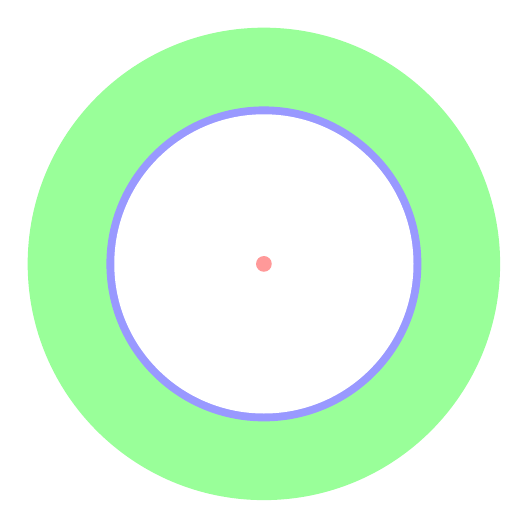
\begin{tikzpicture}
    \fill[green!40!white]  (0,0) circle (3cm);
    \fill[blue!40!white]  (0,0) circle (2cm);
    \fill[white!40!white]  (0,0) circle (1.9cm);
    \fill[red!40!white]  (0,0) circle (0.1cm);
    \end{tikzpicture}

    \caption{Diagram of the simple sphere geometry (not to scale) where the
	blanket is \fcolorbox{white}{green}{\rule{0pt}{6pt}\rule{6pt}{0pt}}, the
first wall is \fcolorbox{white}{blue}{\rule{0pt}{6pt}\rule{6pt}{0pt}} and the
neutron point source is \fcolorbox{white}{red}{\rule{0pt}{6pt}\rule{6pt}{0pt}}.
Blanket and first wall thickness, as well as their material and structural
properties, are adjustable parameters of the simulation that are later optimized
(see~\Tref{tbl:params} for complete parameter listing).}
    \label{fig:model_diagram}
\end{figure}

Paramak facilitates simulation via OpenMC neutronics workflow that is enclosed in
a portable Docker container, which conveniently exposes an HTTP API using the
Python~3 \texttt{flask} package. For the purposes of our work, we used this setup to
simulate a point source with a Muir energy distribution \cite{openmcmuir}\footnotemark[1]
around~\SI{14.06}{\mega\electronvolt} to approximate a Deuterium-Tritium (D-T)
plasma neutron source. Illustrated in~\Fref{fig:model_diagram}, the simulated
geometry was deliberately left adjustable, so that dependency of TBR on various
parameters may be explored. Nuclear data for simulation was extracted from the following sources, in order of preference: FENDL 3.1d \cite{fendl31d}; JEFF 3.3 \cite{jeff33}; and ENDF/B-VII.1 \cite{2011ii}.
To maintain model-agnostic approach, variance reduction (VR) techniques
were not used to accelerate the MC neutronics simulation~\cite{Kleijnen2013}.
It should be noted that depending on application, VR may constitute a viable
alternative to the presented work.

For the remainder of~\Sref{sec:introduction}, we will define the TBR and further motivate our
research. In~\Sref{sec:methodology} we will present our methodologies for the comparison
testing of a wide variety of surrogate modelling techniques, as well as defining the adaptive sampling procedure QASS. After delivering the
results of these approaches in~\Sref{sec:results}, we will give our final conclusions and
recommendations in~\Sref{sec:conclusion}.

\footnotetext[1]{A bug in the Muir distribution involving erronous normal
sampling was recently uncovered (see
\url{https://github.com/openmc-dev/openmc/pull/1670}), but is disregarded in the present approach-focused work.}


\subsection{Problem Description}
\label{sec:problemdescription}

Nuclear fusion technology relies on the production and containment of an
extremely hot and dense plasma containing enriched Hydrogen isotopes. The current frontier generation of fusion reactors, such as the Joint European Torus (JET) and the
under-construction ITER, make
use of both tritium and deuterium fuel. While at least one deuterium atom occurs for every \num{5000} molecules of naturally-sourced water, and may be easily distilled, tritium is extremely rare in nature. It may be produced indirectly through irradiation of heavy water
(\DDO) during nuclear fission, but only at very low rates which could
never sustain industrial-scale fusion power.

Modern D-T reactors rely on tritium breeding blankets, specialized
layers of material which partially line the reactor and produce tritium upon
neutron bombardment, e.g.~by 
\begin{eqnarray}
	\isotope[1][0]{n} + \hspace{3pt} \isotope[6][3]{Li} 
	&\longrightarrow \hspace{3pt} 
	\isotope[3][1]{T} + \hspace{3pt}\isotope[4][2]{He} \\
	\isotope[1][0]{n} + \hspace{3pt} \isotope[7][3]{Li} 
	&\longrightarrow \hspace{3pt} 
	\isotope[3][1]{T} + \hspace{3pt} \isotope[4][2]{He} + \hspace{3pt} \isotope[1][0]{n}
\end{eqnarray}%
where T represents tritium and \isotope[7]{Li}, \isotope[6]{Li} are the more and
less common isotopes of lithium, respectively. The TBR is defined as the ratio of tritium produced per source neutron
, whose description in Paramak is facilitated by 2~classes of parameters
(exhaustively listed in~\Tref{tbl:params}). While the geometry of a given
reactor is described by continuous parameters, material selections are specified
by discrete categorical parameters. For all parameters, we have attempted to cover the full theoretical range of values even where those values are practically infeasible with current technology (e.g. packing fractions close to 1). Simulating broadly around typical values of parameters is necessary to construct the most accurate model of the typical range, and also aids in demonstrating the robustness of constructed models.

In our work, we set out to produce a fast TBR surrogate model, which takes the same input parameters as the MC model used in Paramak and approximates its output with the greatest achievable regression performance, while also minimising the required quantity of expensive-model samples needed for training.

\begin{table}[t]
	\setlength\tabcolsep{2pt}
	\renewcommand{\arraystretch}{0.95}
	\caption{\label{tbl:params}Input parameters supplied to Paramak and surrogates in alphabetical order. Groups of fractions marked\textsuperscript{\textdagger
		\textdaggerdbl} are independently required to sum to 1.}
	\begin{indented}
	\item[]
		\begin{tabular}{l|ll}
		\toprule
		{} & Parameter name (abbreviation) & Domain\\
		\midrule
		\parbox[t]{2mm}{\hspace{-2pt}\multirow{12}{*}{\rotatebox[origin=c]{90}{Blanket}}}
		   & Breeder fraction\textsuperscript{\textdagger} & $[0,1]$\\
		   & Breeder \isotope[6]{Li} enrichment fraction & $[0,1]$\\
		   & Breeder material (BBM) & $\{\text{Li}_2\text{TiO}_3, \text{Li}_4\text{SiO}_4\}$\\
		   & Breeder packing fraction & $[0,1]$\\
		   & Coolant fraction\textsuperscript{\textdagger} & $[0,1]$\\
		   & Coolant material (BCM) & $\{\text{D}_2\text{O}, \text{H}_2\text{O}, \text{He}\}$\\
		   & Multiplier fraction\textsuperscript{\textdagger} & $[0,1]$\\
		   & Multiplier material (BMM) & $\{\text{Be}, \text{Be}_{12}\text{Ti}\}$\\
		   & Multiplier packing fraction & $[0,1]$\\
		   & Structural fraction\textsuperscript{\textdagger} (BSM) & $[0,1]$\\
		   & Structural material & $\{\text{SiC}, \text{eurofer}\}$\\
		   & Thickness & $[0,500]\text{ cm}$\\
		\midrule
		\parbox[t]{2mm}{\hspace{-2pt}\multirow{6}{*}{\rotatebox[origin=c]{90}{First wall}}}
		   & Armour fraction\textsuperscript{\textdaggerdbl} & $[0,1]$\\
		   & Coolant fraction\textsuperscript{\textdaggerdbl} & $[0,1]$\\
		   & Coolant material (FCM) & $\{\text{D}_2\text{O}, \text{H}_2\text{O}, \text{He}\}$\\
		   & Structural fraction\textsuperscript{\textdaggerdbl} & $[0,1]$\\
		   & Structural material (FSM) & $\{\text{SiC}, \text{eurofer}\}$\\
		   & Thickness & $[0,20]\text{ cm}$\\
		\bottomrule
		\end{tabular}
	\end{indented}
	% TODO: verify with JS that thickness unit is indeed cm
\end{table}

